\documentclass[a4paper]{article}
\usepackage{multirow}
\usepackage{longtable}
\usepackage{graphicx}

\begin{document}

\subsubsection{CompareParentsMatched}

  \begin{description}
  \item[testcase\_01] Es werden 2 identische Modelle verglichen.
    
  \textbf{Similarity:} 0
    
	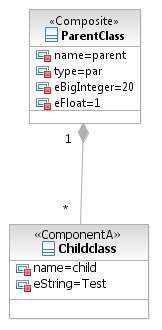
\includegraphics[scale=0.9]{CompareParentsMatchedOrSimilarTestScreens/Testcase01model1.jpeg}
	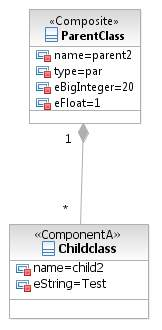
\includegraphics[scale=0.9]{CompareParentsMatchedOrSimilarTestScreens/Testcase01model2.jpeg}

  \item[testcase\_02] Es werden 2 identische Modelle verglichen.
    
  \textbf{Similarity:} 1
    
	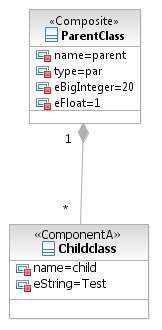
\includegraphics[scale=0.9]{CompareParentsMatchedOrSimilarTestScreens/Testcase01model1.jpeg}
	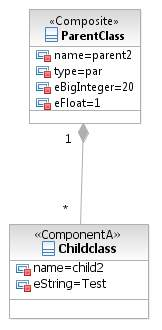
\includegraphics[scale=0.9]{CompareParentsMatchedOrSimilarTestScreens/Testcase01model2.jpeg}

  \item[testcase\_03] Es werden 2 Modelle, die sich bei den Eltern in Anzahl und Wert der Attribute unterscheiden, verglichen.
    
  \textbf{Similarity:} 0
    
	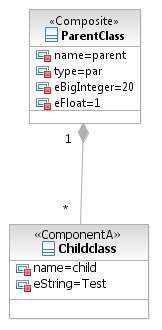
\includegraphics[scale=0.9]{CompareParentsMatchedOrSimilarTestScreens/Testcase03model1.jpeg}
	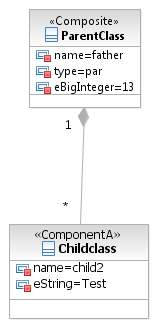
\includegraphics[scale=0.9]{CompareParentsMatchedOrSimilarTestScreens/Testcase03model2.jpeg}

  \item[testcase\_04] Es werden 2 Modelle, die sich bei den Eltern in Anzahl und Wert der Attribute unterscheiden, verglichen.
    
  \textbf{Similarity:} 1
    
	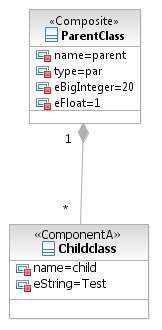
\includegraphics[scale=0.9]{CompareParentsMatchedOrSimilarTestScreens/Testcase03model1.jpeg}
	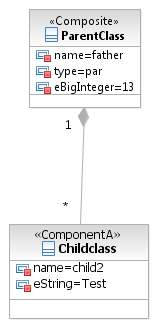
\includegraphics[scale=0.9]{CompareParentsMatchedOrSimilarTestScreens/Testcase03model2.jpeg}

  \item[testcase\_05] Es werden 2 Modelle, die sich bei den Kindattributen unterscheiden, verglichen.
    
  \textbf{Similarity:} 0
    
	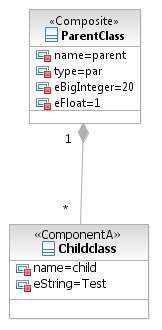
\includegraphics[scale=0.9]{CompareParentsMatchedOrSimilarTestScreens/Testcase05model1.jpeg}
	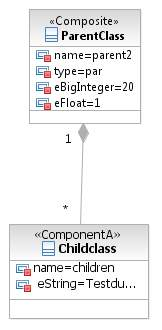
\includegraphics[scale=0.9]{CompareParentsMatchedOrSimilarTestScreens/Testcase05model2.jpeg}

  \item[testcase\_06] Es werden 2 Modelle, die sich bei den Kindattributen unterscheiden, verglichen.
    
  \textbf{Similarity:} 1
    
	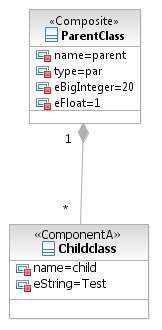
\includegraphics[scale=0.9]{CompareParentsMatchedOrSimilarTestScreens/Testcase05model1.jpeg}
	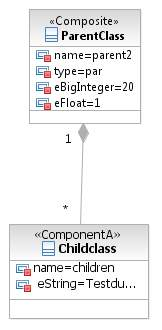
\includegraphics[scale=0.9]{CompareParentsMatchedOrSimilarTestScreens/Testcase05model2.jpeg}

  \item[testcase\_07] Es werden 2 v�llig unterschiedliche Modelle verglichen.
    
  \textbf{Similarity:} 0
    
	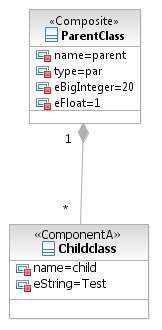
\includegraphics[scale=0.9]{CompareParentsMatchedOrSimilarTestScreens/Testcase07model1.jpeg}
	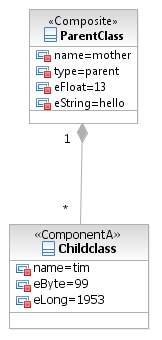
\includegraphics[scale=0.9]{CompareParentsMatchedOrSimilarTestScreens/Testcase07model2.jpeg}

  \item[testcase\_08] Es werden 2 v�llig unterschiedliche Modelle verglichen.
    
  \textbf{Similarity:} 1
    
	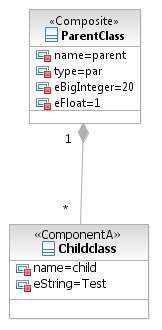
\includegraphics[scale=0.9]{CompareParentsMatchedOrSimilarTestScreens/Testcase07model1.jpeg}
	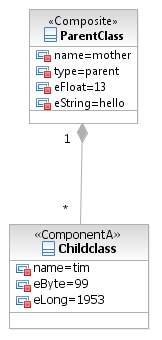
\includegraphics[scale=0.9]{CompareParentsMatchedOrSimilarTestScreens/Testcase07model2.jpeg}
	\end{description}
	
	



\end{document}